\section{Esempi di lavorazione}
Mostriamo ora alcuni esempi di lavorazione, per vedere come i tempi di esecuzione catalogati variano a seconda dei parametri scelti.

Le prove sono state effettuate usando i due file messi a disposizione per i testing, uno con oltre 7000 posizioni, e l'altro con oltre 20000. I tempi riportati si riferiscono a test effettuati usando una macchina con Ubuntu Linux 12.04 a 64 bit, con processore Intel i7 a 1.73 GHz e 4GB di RAM, con il simulatore compilato in modalità \verb!release!. Per la profilazione invece si è reso necessario compilare on modalità \verb!debug!. Abbiamo effettuato varie prove per ciascuna configurazione, e abbiamo qui riportato i valori medi.

\subsection{Modalità testuale}
Vediamo innanzitutto (tabelle \ref{tab:positionsnone} e \ref{tab:positions2none}) come si comporta il simulatore quando viene eseguito in modalità solo testuale.

\begin{center}
  \begin{table}[h]
    \begin{minipage}{.5\linewidth}
      \vspace{0pt}
      \begin{tabular}{ccc}
        \toprule
          \shortstack{Dimensione\\ Voxel} & \shortstack{Tempo \\\texttt{[s]}} & \shortstack{Memoria \\\texttt{[MiB]}}\\
        \midrule
          3   & 0.517  & -\footnote{termina troppo presto perché io riesca a vedere quanto occupa... TODO spiegare in maniera potabile sta roba - o trovare una maniera per leggere quanto occupa prima che la riga sparisca dal monitor di sistema}     \\
          2.5 & 0.543  & -     \\
          2   & 1.632  & 17.2  \\
          1.5 & 1.607  & -     \\
          1   & 8.437  & 70.0  \\
          0.5 & 67.691 & 334.7 \\
        \bottomrule
      \end{tabular}
      \caption{Test con file \texttt{positions.txt}.}
      \label{tab:positionsnone}
    \end{minipage}
    \begin{minipage}{.5\linewidth}
      \vspace{0pt}\raggedright
      \begin{tabular}{ccc}
        \toprule
          \shortstack{Dimensione\\ Voxel} & \shortstack{Tempo \\\texttt{[s]}} & \shortstack{Memoria \\\texttt{[MiB]}}\\
        \midrule
          3   & 2.446   & 22.7   \\
          2.5 & 2.558   & 12.2   \\
          2   & 11.478  & 90.6   \\
          1.5 & 11.613  & 95.0   \\
          1   & 99.785  & 463.4  \\
          0.5 & 973.191 & 2764.8\footnote{ha swappato, non so se per il monitor di sistema cambi qualcosa.} \\
        \bottomrule
      \end{tabular}
      \caption{Test con file \texttt{positions2.txt}.}
      \label{tab:positions2none}
    \end{minipage}
    %\caption{Riepilogo dei test effettuati in modalità testuale.}
    %\label{tab:graphicsnone}
  \end{table}
\end{center}

Vediamo come con voxel grandi i tempi di esecuzione sono molto ridotti e molto simili, con poca occupazione di memoria, mentre con voxel più piccoli i tempi crescono compatibilmente con un fattore 8 (l'arietà dell'Octree). Questo è segno che con voxel grandi l'albero generato è poco profondo e viene analizzato molto velocemente, con un impatto poco significativo sul tempo di esecuzione totale. Al diminuire della dimensione dei voxel, l'Octree è invece più profondo, e la sua scansione occupa una parte sempre più consistente del tempo di esecuzione totale.% In particolare, l'albero generato usando il file \texttt{positions2.txt} genera un albero quasi completo.

\subsection{Modalità grafica \texttt{box}}
La modalità grafica \texttt{box} è la modalità che non utilizza l'algoritmo MarchingCubes per il taglio dei voxel, ma usa l'oggetto \texttt{Box} di OpenSceneGraph per rappresentare ciascun voxel.

\subsection{Modalità grafica \texttt{mesh}}
La terza modalità di visualizzazione è quella che utilizza l'algoritmo MarchingCubes per estrarre la mesh tridimensionale dai voxel.

\subsection{Confronto tra \texttt{box} e \texttt{mesh}}
Mettiamo ora a confronto la visualizzazione della lavorazione con la modalità di visualizzazione \texttt{box} e la modalità \texttt{mesh} (le immagini sono zoomate per apprezzare le differenze).
\begin{center}
\begin{table}[h]
  \begin{tabular}{cc}
   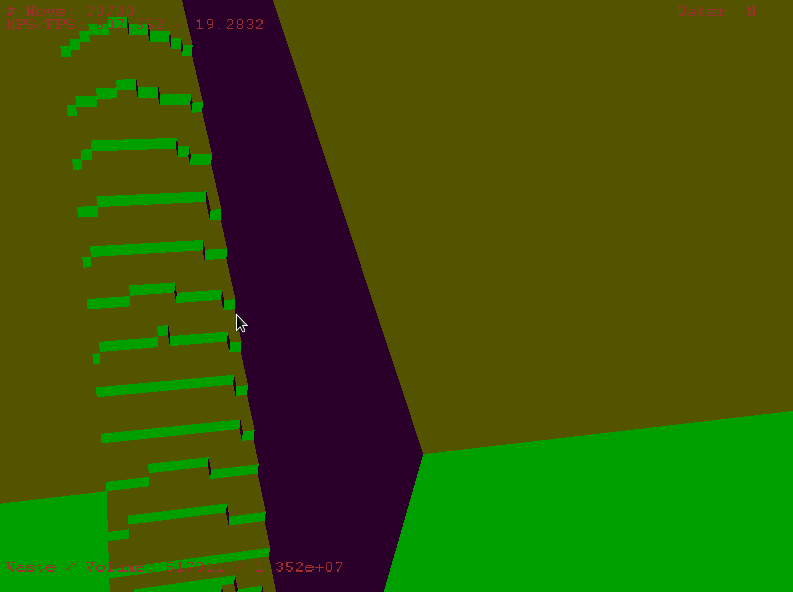
\includegraphics[width=0.48\textwidth]{img/screenshots/pos2_box_v2_2.png} &%
   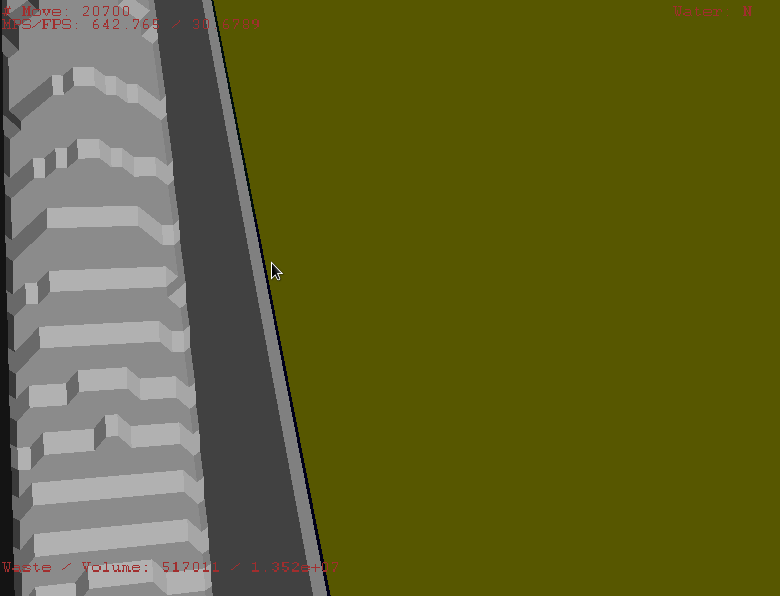
\includegraphics[width=0.48\textwidth]{img/screenshots/pos2_mesh_v2_2.png}\\
  \end{tabular}
  \caption{Confronto tra modalità \texttt{box} e modalità \texttt{mesh} con dim. voxel pari a $2$.}
  \label{tab:confrontobm1}
\end{table}
\end{center}

In \ref{tab:confrontobm1} vediamo la differenza nell'approssimazione della fresatura da parte del cilindro in modalità \texttt{box} (a sx) e \texttt{mesh} (a dx) con dimensione minima dei voxel pari a $2$. Vediamo come, nella modalità \texttt{mesh}, l'algoritmo MarchingCubes approssimi meglio la lavorazione, pur mantenendo visibile la struttura ``a cubi'' del rendering.

\begin{center}
\begin{table}[h]
  \begin{tabular}{cc}
   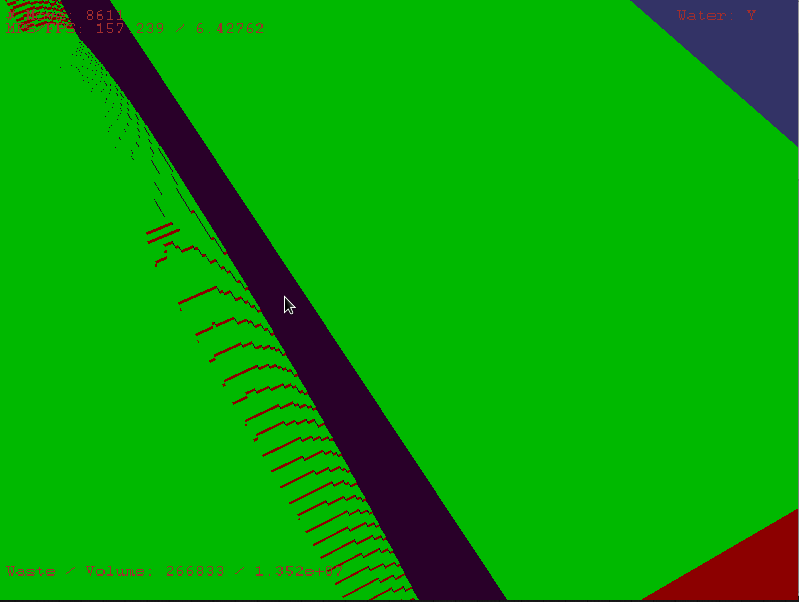
\includegraphics[width=0.48\textwidth]{img/screenshots/pos2_box_v1.png} &%
   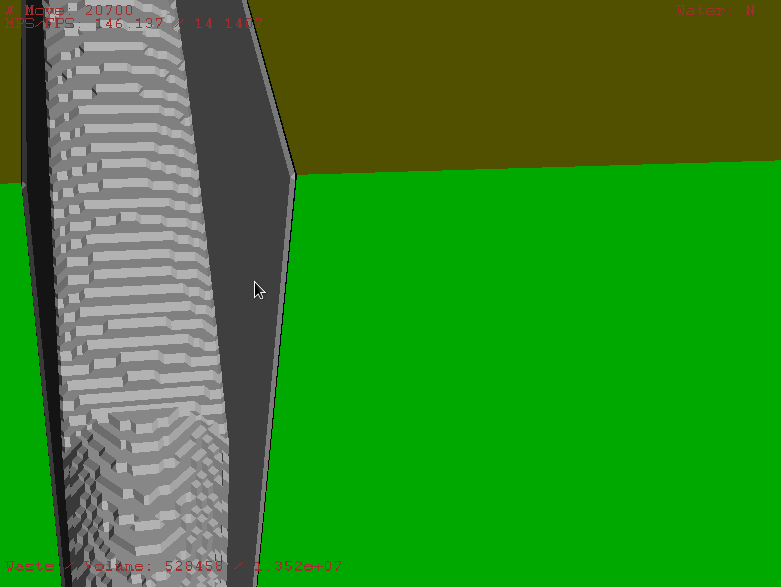
\includegraphics[width=0.48\textwidth]{img/screenshots/pos2_mesh_v1_2.png}\\
  \end{tabular}
  \caption{Confronto tra modalità \texttt{box} e modalità \texttt{mesh} con dim. voxel pari a $1$.}
  \label{tab:confrontobm2}
\end{table}
\end{center}

\begin{center}
\begin{table}[h]
  \begin{tabular}{cc}
   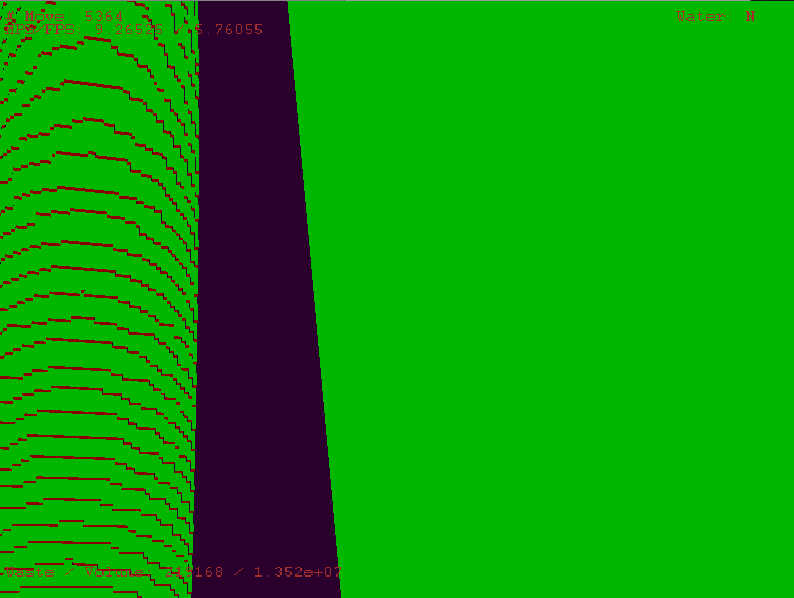
\includegraphics[width=0.48\textwidth]{img/screenshots/pos2_box_v05.png} &%
   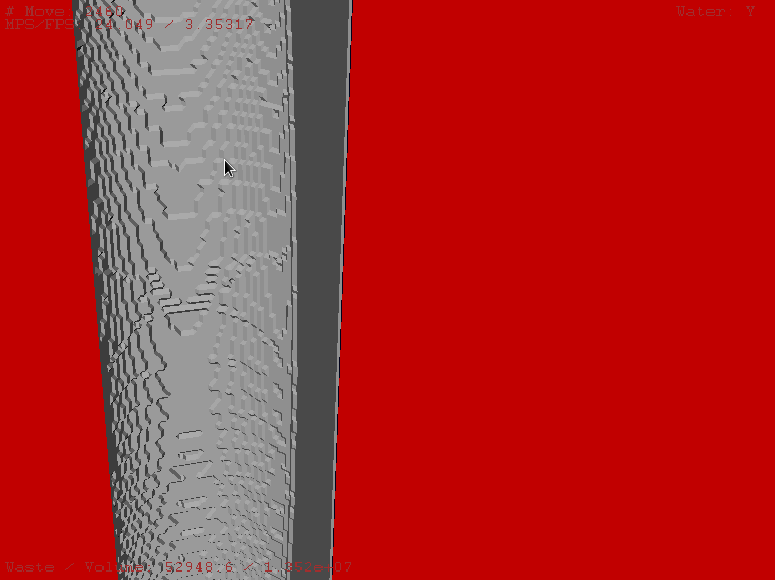
\includegraphics[width=0.48\textwidth]{img/screenshots/pos2_mesh_v05.png}\\
  \end{tabular}
  \caption{Confronto tra modalità \texttt{box} e modalità \texttt{mesh} con dim. voxel pari a $0.5$.}
  \label{tab:confrontobm3}
\end{table}
\end{center}

In \ref{tab:confrontobm2} e \ref{tab:confrontobm3} invece vediamo la stessa lavorazione, effettuata con dimensione dei voxel pari a, rispettivamente, $1$ e $0.5$. Vediamo come man mano che la dimensione dei voxel diminuisce, entrambe le modalità, ovviamente, approssimano in maniera sempre più precisa la fresatura. Tuttavia, mentre la modalità \texttt{box} approssima la lavorazione in modo sempre più preciso ma rimane comunque visibile la quadrettatura, l'algoritmo MarchingCubes che lavora alla stessa profondità dell'Octree fornisce risultati sempre più precisi e realistici.

Vediamo, invece, dalle tabelle seguenti (\ref{tab:positionsBox} $\div$ \ref{tab:positions2Mesh}) come l'implementazione con MarchingCubes sia più veloce, seppur di poco, in lavorazioni veloci e che comportino la generazione di un Octree poco bilanciato e poco profondo. All'aumentare della profondità dell'albero, invece, la semplicità della generazione dei \texttt{Box} di OSG risulta più veloce. Per lavorazioni più complesse, che richiedono un Octree più completo, l'approccio \texttt{box} è più veloce rispetto alla generazione della \texttt{mesh} in tutti i test effettuati.

\begin{center}
  \begin{table}[h]
    \begin{minipage}{.5\linewidth}
      \vspace{0pt}
      \begin{tabular}{ccc}
        \toprule
          \shortstack{Dimensione\\ Voxel} & \shortstack{Tempo \\\texttt{[s]}} \\
        \midrule
          3   & - \\
          2.5 & - \\
          2   & 2.090 \\
          1.5 & 2.093 \\
          1   & 10.267 \\
          0.5 & 81.466 \\
        \bottomrule
      \end{tabular}
      \caption{Test sul file \texttt{positions.txt} in modalità \texttt{box}.}
      \label{tab:positionsBox}
    \end{minipage}
    \begin{minipage}{.5\linewidth}
      \vspace{0pt}\raggedright
      \begin{tabular}{ccc}
        \toprule
          \shortstack{Dimensione\\ Voxel} & \shortstack{Tempo \\\texttt{[s]}}\\
        \midrule
          3   & - \\
          2.5 & -  \\
          2   & 1.988  \\
          1.5 & 1.971 \\
          1   & 9.807  \\
          0.5 & 94.821 \\
        \bottomrule
      \end{tabular}
      \caption{Test sul file \texttt{positions.txt} in modalità \texttt{mesh}.}      \label{tab:positionsMesh}
    \end{minipage}
    %\caption{Riepilogo dei test effettuati in modalità testuale.}
    %\label{tab:graphicsnone}
%   \end{table}
% \end{center}

% \begin{center}
%   \begin{table}[h]
    \begin{minipage}{.5\linewidth}
      \vspace{0pt}
      \begin{tabular}{ccc}
        \toprule
          \shortstack{Dimensione\\ Voxel} & \shortstack{Tempo \\\texttt{[s]}} \\
        \midrule
          3   & 2.381 \\
          2.5 & 2.510 \\
          2   & 12.719  \\
          1.5 & 12.581 \\
          1   & 126.827 \\
          0.5 & arriva... \\
        \bottomrule
      \end{tabular}
      \caption{Test sul file \texttt{positions2.txt} in modalità \texttt{box}.}
      \label{tab:positions2Box}
    \end{minipage}
    \begin{minipage}{.5\linewidth}
      \vspace{0pt}\raggedright
      \begin{tabular}{ccc}
        \toprule
          \shortstack{Dimensione\\ Voxel} & \shortstack{Tempo \\\texttt{[s]}}\\
        \midrule
          3   & 2.690 \\
          2.5 & 2.581 \\
          2   & 16.221 \\
          1.5 & 19.051 \\
          1   & 127.073 \\
          0.5 & 1684.734 \\
        \bottomrule
      \end{tabular}
      \caption{Test sul file \texttt{positions2.txt} in modalità \texttt{mesh}.}
      \label{tab:positions2Mesh}
    \end{minipage}
  \end{table}
\end{center}
